%%
%% Template intro.tex
%%

\chapter{Introduction}
\label{cha:intro}

The night sky has always been a source of wonder since the dawn of recorded history.
Even before the discovery of the scientific method, we used our built-in pattern
recognition and tried to assign a purpose to
the cosmos with stories of gods and the supernatural. Then came the Ancient Greeks who brought
mathematics to astronomy and sought a more rational explanation of celestial bodies.
But we could only discover so much with our naked eyes. It was not until the invention
of new technology during the Scientific Revolution like the telescope that we began to
make significantly more progress. And yet, 400 years after Galileo made the first working
telescope, most of the sky still remains unknown to us.

This, however, is starting to change. The Sloan Digital Sky Survey (SDSS) began
in 2000 and has since obtained 800 million sets of photometric measurements
and 3 million spectra of the northern sky. Similar projects are going on
to map the southern sky including the VST-ATLAS. We now face another challenge of how
to analyse this huge amount of data. Fortunately, we can bring machine learning
to astronomy and let the computer to do the pattern recognition task.

This thesis is an attempt to study a small part of the interaction between these
two disciplines, in particular how we can effectively use multi-arm bandit active
learning to select a good training set. Along the way, we will build an open-source
Python package that allows practitioners to apply the algorithms described in this thesis
to real-world data out of the box. In our own experiments, we will use the SDSS and the
VST-ATLAS datasets to evaluate the performance.



\section{Spectroscopy and Photometry}
\label{sec:spec}

When many people think about astronomy, the first things that pop into their mind are
breathtaking images of the sky like the famous Hubble Deep Field. But pretty images alone
are not enough to do real science. For us to make any meaningful observations about
astronomical objects, we need actual quantitative measurements.

One such quantitative approach is spectroscopy. This involves
using diffraction grating to disperse light and measure the amount of electromagnetic radiation,
or flux, emitted from an object at small wavelength intervals. As the name implies, we end
up with a spectrum, like the one shown in Figure \ref{fig:vega}. The shape of the spectrum
and its absorption lines allow us to deduce many useful properties such as the object's
temperature and chemical composition.

Unfortunately, it can be very costly to take high resolution spectra of faint objects since
we are spreading light thinly across many wavelengths. To get around this problem, we need
to separate light into fewer groups. Indeed this is what we do in photometry, a method
that is much cheaper and faster than spectroscopy.

In photometry, we have a set of filters, each of which can be put in front of the CCD
camera to allow only light from certain wavelengths to pass through. Associated with
each filter is a transmission function $T(\lambda)$ that tells us
the fraction of light that the filter will transmit at wavelength $\lambda$.
Figure \ref{fig:vega} shows $T(\lambda)$ of the five bandpasses (u, g, r, i, and z) that
are used in the SDSS.


\begin{figure}[tbp]
	\centering
	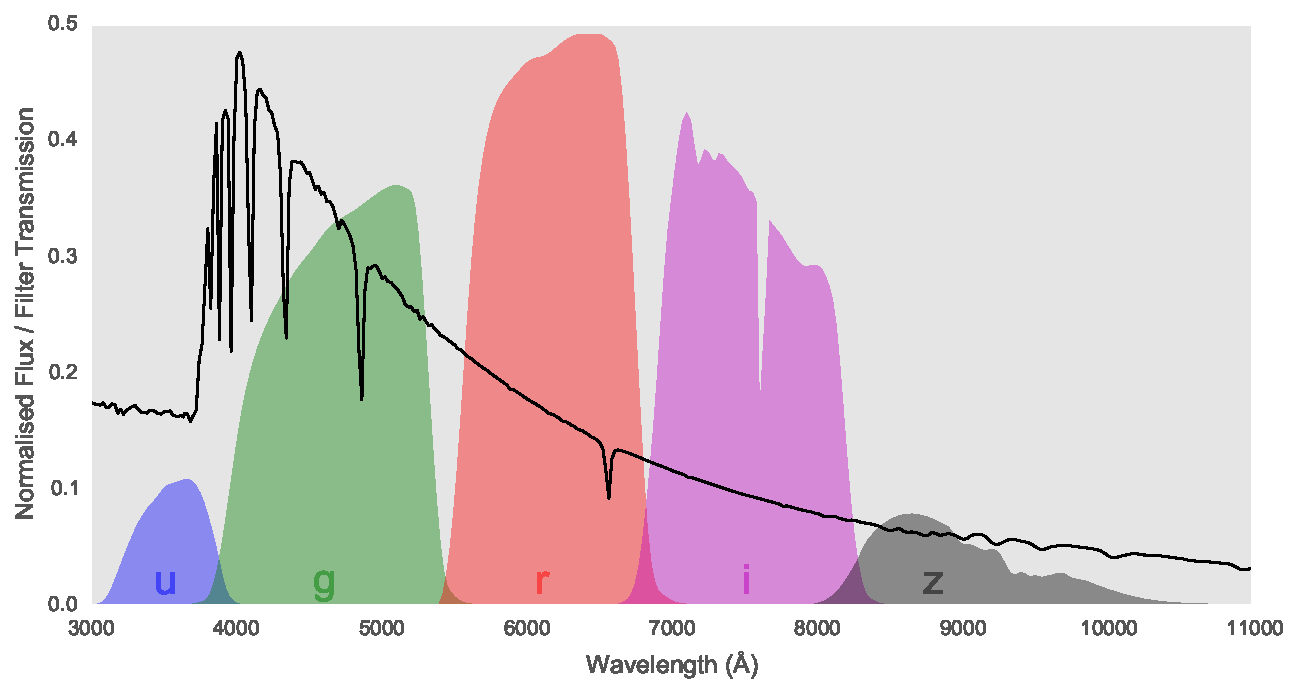
\includegraphics[width=\textwidth]{figures/vega_filters_and_spectrum}
	\caption[The spectrum of the star Vega and the ugriz band passes]{The spectrum of Vega
		(the fifth brighest star in the night sky) and the ugriz bandpasses used in the SDSS.}
	\label{fig:vega} \index{Vega}
\end{figure}


\section{Measuring Fluxes and Magnitudes}
\label{sec:mag}
When light hits the CCD, all we have initially are counts of photons, one for each pixel.
The first challenge is to assign the photons to distinct objects. Two models are used
in the SDSS, depending on whether we assume the object is an extended source or a point source.


\subsection{Petrosian Flux}

Galaxies are extended-source objects so we need to define an aperture radius, within which
all the photons are added together to obtain the flux of the galaxy. However galaxies have
poorly defined edges, so we need a consistent method to pick the aperture radius. \shortciteN{blanton01} define a quantity called the Petrosian ratio:
	\begin{IEEEeqnarray*}{lCl}
		\mathfrak{R}_p(r) = \frac{\int_{0.8r}^{1.25r} 2\pi s I(s) \, ds}{\pi (1.25^2 - 0.8^2) r^2}
							\bigg/ \frac{\int_0^r 2\pi s I(s) \, ds}{\pi r^2}
	\end{IEEEeqnarray*}
This is the ratio of the mean local surface brightness over an annulus at $r$ to the mean
surface brightness within $r$. The quantity $I(r)$ is the galaxy surface brightness profile
and can be estimated from the photon count. With this, we define the Petrosian
radius $r_p$ as the radius such that $\mathfrak{R}_p(r_p) = 0.2$. This is one of the features
in the SDSS dataset that will prove to be very useful in distinguishing galaxies from
point-source objects. The aperture radius is then chosen to be $2r_p$ to ensure that almost
all of the light from a typical galaxy is captured. Finally for each bandpass, we can calculate
the corresponding Petrosian flux as
	\begin{IEEEeqnarray*}{lCl}
		f &=& \int_{0}^{2 r_p} 2 \pi s I(s) \, ds
	\end{IEEEeqnarray*}

\subsection{Point Spread Function Fitting}
Stars and quasars are unresolved point sources so they can be modelled by a point
spread function (PSF). This approach is particularly useful when we examine a dense region
like a globular cluster. In such places, given the amount of overlap, it would be very
difficult define an aperture that includes only photons from an object and excludes all others
from the neighbours. In PSF fitting, we assume that all objects have the same shape and fit
a Gaussian model to each of them. We then iteratively vary the position and flux of the objects
until the model produces the observed light distribution \cite{palmer01}.


\subsection{Magnitudes}

We will not use fluxes themselves as features. Instead, we convert them to inverse
hyperbolic sine (or arsinh) magnitudes:
	\begin{IEEEeqnarray*}{lCl}
		m &=& -\frac{2.5}{\ln(10)} \Bigg[ \arsinh\bigg(\frac{f/f_0}{2b}\bigg) + \ln(b) \Bigg]
	\end{IEEEeqnarray*}
Here $f_0$ is the flux of the object with a conventional magnitude of 0 and $b$ is the
the softening parameter. A nice feature of the magnitude system is its logarithmic scale--with
every decrease of 1 in the magnitude scale, the object becomes 2.5 times brighter.\footnote{
	The reader might wonder why the scale works in reverse, with a small magnitude
	corresponding to more brightness. This is the convention created two centuries ago by
	the Greek astronomer Hipparchus, which, for better or worse, has stuck with us ever since.}



\section{Machine Learning}
\label{sec:machine}

The SDSS dataset contains photometric observations of 800 million objects. Each object
has 11 measurements: a Petrosian magnitude and a PSF magnitude for each of the five
ugriz bands, along with the Petrosian radius in the r-band. In the most basic
classification task, we would like to assign a label (star, galaxy, or quasar) to each object.
To manually classify them using only photometric data would very difficult, due to the 
sheer volume of data and the fact that we only have 11 numbers to work with. Astronomers, however,
are very good at spectroscopic classification, since a spectrum contains a lot more
information in them. But spectra are expensive to obtain. In the SDSS, we only have just under
3 million spectra.

The good news is that this is a very well-studied problem in machine learning...

\subsection{Random Forest}

\subsection{Logistic Regression}

\subsection{Support Vector Machines}




\section{Active Learning}
\label{sec:organisation}

%%% Local Variables: 
%%% mode: latex
%%% TeX-master: "thesis"
%%% End: 
